\documentclass[../main.tex]{subfiles}
\begin{document}

The Jaccard index is a standard measure of similarity for categorical datasets. Some classical use cases include text analysis in the form of document clustering and search engine result refinement \cite{broder1997syntactic}, source code plagiarism detection \cite{moussiades2005pdetect}, and as a loss function in machine learning tasks related to medical image segmentation \cite{yuan2017automatic}. By discretizing the location data of our mobile network trajectories, we've essentially turned each trajectory into a list of tokens, not unlike documents of text, where each location and time entry becomes a word in a very large alphabet. Since the Jaccard index typically shines when it comes to similarity searches in very large text corpora it seems a natural choice for experimentation with these kinds of trajectory representations.

\section{Definitions}
Lets for a moment consider the binary case $r_1,r_2\subset 2^\mathcal{A} \times \mathbf{T}$ for some time-discretization $\mathbf{T} = \{0,1,2,\dots,n\}$. For each timestamp $t\in\mathbf{T}$, let $A_t, B_t \in 2^\mathcal{A}$ be the sets of antennas that the trajectories $r_1$ and $r_2$ connected with at that time. Taking the cardinality of the symmetric set difference $|A_t \triangle B_t|$ between $A_t$ and $B_t$ provides a simple way to compare how many of the antennas each trajectory have in common. The assumption here being that two devices are closer in space if they connect to the same antennas at the same time. Then, since each set is finite and by applying a normalization factor
\begingroup
\addtolength{\jot}{1em}
\begin{align*}
    \frac{|A_t \triangle B_t|}{|A_t \cup B_t|} &= \frac{|(A_t\cup B_t) \setminus (A_t\cap B_t)|}{|A_t \cup B_t|} \\
    &= \frac{|(A_t\cup B_t)| - |(A_t\cap B_t)|}{|A_t \cup B_t|} \\
    &= 1 - \frac{|A_t \cap B_t|}{|A_t \cup B_t|}
\end{align*}
\endgroup
This last expression is known in the literature as the Jaccard distance. The ratio of the intersection over union is the Jaccard index
$$
J(A,B) = \frac{|A \cap B|}{|A \cup B|}.
$$
In this case we've only compared two single datapoints, but borrowing from the Euclidean lock-step method we define
$$
d_J(r_1, r_2) = 1 - \frac{1}{n}\sum_{t=0}^nJ(A_t, B_t)
$$
as a rough measure of trajectory similarity. The idea can be extended to co-trajectories $R_1 = \{r_{1,i}\}_{i=1}^N$ and $R_2 = \{r_{2,j}\}_{j=1}^M$ by taking the union of all datapoints at time $t$ over all trajectories in the co-trajectory.
$$
d_J(R_1, R_2) = 1 - \frac{1}{n}\sum_{t=0}^nJ(\bigcup_{i=1}^NA_{t,i},\bigcup_{j=1}^MB_{t,j})
$$
where $A_{t,i}$ is the set of antennas that the trajectory $r_{1,i} \in R_1$ connected with at time $t$, and likewise for $B_{t,j}$ with $ r_{2,j} \in R_2$. 

However for large enough co-trajectories we quickly run into a problem. Since the Jaccard index disregards all information about connection frequencies it cannot differentiate between co-trajectories based on the number of times connections are established. If enough devices within a geographic area are included then it is very likely that every available antenna is connected to at least one device from each co-trajectory, making
them equal.

To account for this we instead look at the \textit{generalized} or \textit{weighted} Jaccard index $J_W(A,B)$, defined as
$$
J_W(A,B) = \frac{\sum_imin(a_i,b_i)}{\sum_imax(a_i,b_i)}
$$
where are two weighted sets, or multi-sets. Then by considering again trajectories $r_1,r_2 \subset \{(\mathcal{A}, m):m\in\mathbb{N}^\mathcal{A}\}\times\mathbf{T}$ we redefine the distance measure as
$$
d_J(r_1, r_2) = 1 - \frac{1}{n}\sum_{t=0}^nJ_W((\mathcal{A}, m_t), (\mathcal{A}, p_t))
$$
and
$$
d_J(R_1, R_2) = 1 - \frac{1}{n}\sum_{t=0}^nJ_W(\sum_{i=1}^N(\mathcal{A}, m_{t,i}),\sum_{j=1}^M(\mathcal{A}, p_{t,j}))
$$
for a family of functions $m_{t,i}, p_{t,j}: \mathcal{A} \rightarrow \mathbb{N}$ where the sum of two multi-sets is defined as
\begin{align*}
    (A,m) + (A,p) &=  \{a_1^{m(a_1)},a_2^{m(a_2)},\dots, a_n^{m(a_n)}\} + 
    \{a_1^{p(a_1)},a_2^{p(a_2)},\dots, a_n^{p(a_n)}\} \\
    &= \{a_1^{m(a_1) + p(a_1)}, a_2^{m(a_2) + p(a_2)},\dots, a_n^{m(a_n) + p(a_n)}\}
\end{align*}
\begin{figure*}[h]
\centering
\begin{adjustbox}{center}
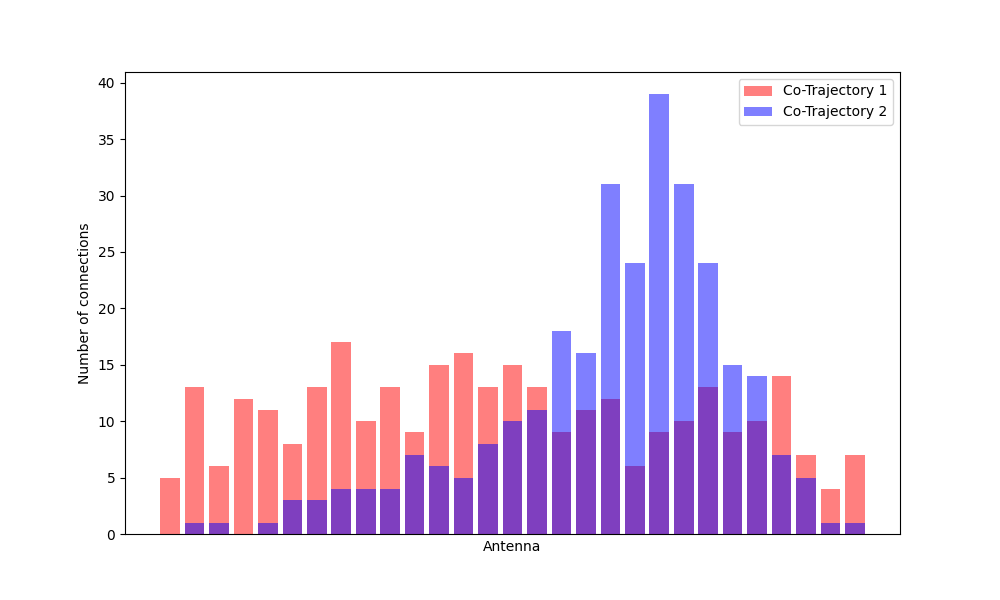
\includegraphics[width=0.98\textwidth]{graphics/non-results/non-weighted.png}
\end{adjustbox}
\caption{Two Co-Trajectories that would be nearly identical under the regular Jaccard distance can nevertheless have very different connection frequencies.}
\end{figure*}
\\
Before implementing this metric and testing it on real-life mobile network data we will spend the next section looking into some approximation algorithms for the weighted Jaccard index. Foremost of all, the MinHash algorithm.

\section{Locality Sensitive Hashing Techniques}


Locality Sensitive Hashing (LSH) is a technique used to perform probabilistic dimension reduction of high dimensional data. Items that are similar, according to some measure, are grouped together into the same buckets with high probability. The buckets are represented by hash values, outputs of a hash function, which is a mathematical function taking variable inputs of arbitrary length and mapping them to outputs of fixed length. The input, called a key, is usually some kind of data, a record, or a string, which the function maps to an output called the hash value. Normally, hash functions are often characterized by their efficiency and minimization of collisions, meaning that distinct keys rarely map to the same hash-value, but in the case of LSH algorithms we are instead interested in maximizing collisions.


\begin{definition}[Locality Sensitive Hashing Scheme \cite{charikar2002similarity}]
    Let $U$ be a set with some defined similarity function $\phi:U\times U\rightarrow [0,1]$ A Locality Sensitive Hashing (LSH) -scheme is a distribution $D$ on a family of hash functions $H$ over $U$ such that for any two objects $x,y\in U$
    $$\textbf{Pr}_{h\in H}[h(x) = h(y)] = sim(x,y)$$
\end{definition}

This simply means that the probability of a hash collision between two objects is equal to their similarity. While there is no agreed upon definition of a similarity function it is easy to see them as a sort of
inverse to ordinary distance measures, but counting 0 as distant instead of close. Further, they are typically bounded in the range $[0,1]$ and it is useful if $1 - sim$ is an ordinary metric, satisfying the usual triangle inequality property, but this does not have to be the case. For our purposes there exists a ready LSH scheme for the Jaccard index.

\begin{definition}[MinHash]
Given a set $U$ and a subset $S \subset U$ let $H$ be a family of real-valued, random and uniform hash functions $h:U\rightarrow [0,1]$. The elements $x\in S$ which are given the minimum hash values $$MHS(S) = \{argmin_x (h(S))\ | h \in H\}$$ are called the MinHashes of $S$.
\end{definition}

The probability that two sets $S,T\in U$ generate the same MinHash values is equal to the Jaccard index 

\begin{theorem}
    Let $U$ and $H$ be defined as before. If $A,B\in U$ then  
    $$Pr_{h\in H}[argmin_x(h(A)) = argmin_x(h(B))] = J(A,B)$$
\end{theorem}
\begin{proof}
    Since each hash function $h\in H$ is uniformly and independently distributed, every element in $A$ and $B$ have an equal and independent chance of being mapped to the minimum value. If $A$ and $B$ share a MinHash $x$ then $x \in A \cap B$. The probability of this element being picked is exactly the Jaccard index.
\end{proof}

Similarly, there are extensions which also works for the weighted Jaccard index. The most important of them being the CWS-scheme
 
\begin{definition}[Consistent Weighted Sampling \cite{manasse2010consistent}.]
Given a weighted set $S = (S_1, \ldots S_n)$ where $S_k \geq 0$ for $k \in \{1,\ldots n\}$ generate a sample $k,y_k$ where $0 \leq y_k \leq S_k$ such that it is uniform and consistent

\begin{itemize}
    \item \textbf{Uniformity:} The sample $(k,y_k)$ is uniformly sampled from $\bigcup_i(\{i\}\times[0,i])$
    \item \textbf{Consistency:} 
    Given two non-empty weighted sets $S$ and $T$ if $\forall k, T_k \leq S_k$ then whenever $(k,y_k)$ satisfying $y_k \leq T_k$ is chosen from $S$ then $(k,y_k)$ is also chosen from $T$
\end{itemize}
\end{definition}

\begin{theorem}[Weighted MinHash \cite{manasse2010consistent}]
    Any sampling scheme $CWS$ which is uniform and consistent satisfies the following property
    $$Pr[CWS(S) = CWS(T)] = J_W(S,T)$$
\end{theorem}
\begin{proof}
    Consider weights $R_k = max(S_k, T_k)$. By consistency, samples from $S$ and $T$ coincide when the sample $(k,y_k)$ from $R$ satisfies $y \leq min(S_k, T_k)$. By uniformity, this happens with the stated probability. 
\end{proof}

Many efficient algorithms have been developed to calculated weighted MinHash samples \cite{wu2020review}, the most influential one being based on the CWS scheme \cite{manasse2010consistent} which reduced the computational complexity through the use of special active indices, allowing constant sampling times independent of the weights themselves, something that had been a problem in earlier, quantization based methods \cite{gollapudi2006exploiting}, especially for real-valued data. 

Several improvements have since been made to the CWS algorithm, including ICWS \cite{ioffe2010improved}, 0-bit CWS \cite{li20150}, CCWS \cite{wu2016canonical}, PCWS \cite{wu2017consistent} and I$^2$CWS \cite{wu2018improved}. In the next section we will explore the use of the I$^2$CWS algorithm as a means to generate MinHashes for trajectory data.

\newpage

\section{I$^2$CWS and Apache Spark}
In this section we present the I$^2$CWS (Improved-Improved Consistent Weighted Sampling) as introduced in \cite{wu2018improved} and discuss an implementation using Apache Spark, an open-source distributed analytics engine that is widely used in industry for processing large datasets.
Spark is originally written in Scala but provides language APIs for multiple other languages such as Python, Java, R and SQL. In this paper we decided to work in PySpark, the Python API, since it allows teams with Python experience to work with the code. The main working abstraction in Spark is given by the DataFrame API. A DataFrame is a distributed collection of data, a table organized into named columns.
Using Sparks many built-in functions we can easily perform progressive transformations and aggregations on DataFrames. However, for more specialized tasks you can also register user defined functions. We begin by presenting the full I$^2$CWS algorithm and some implementation details.

\begin{algorithm}
\DontPrintSemicolon
\setstretch{1.25}
\caption{The I$^2$CWS algorithm \cite{wu2018improved}}
\label{alg:1}
\KwData{$S = \{S_1, \ldots, S_n\}$}
\KwResult{$(k_*,y_{k_*})$}
\For{$k = 1,\ldots,n$}{
$r_{k_1},r_{k_2} \sim Gamma(2,1)$\;
$\beta_{k_1},\beta_{k_2} \sim Uniform(0,1)$\;
$c_k \sim Gamma(2,1)$
}
\For{for all k such that $S_k > 0$}{
$t_{k2} = \lfloor lnS_k/r_{k_2} + \beta_{k_2}\rfloor$\;
$z_k = exp(r_{k_2}(t_{k_2} - \beta_{k_2} + 1))$\;
$a_k = c_k/a_k$
}
$k_* = argmin_ka_k$\;
$t_{k_*1} = \lfloor ln S_{k_*} / r_{k_*1} + \beta_{k_*1}\rfloor$\;
$y_{k_*} = exp(r_{k_*1}(t_{k_*1} - \beta_{k_*1}))$\;
\Return{$(k_*,y_{k_*})$}
\end{algorithm}

The input $S$ is a vector of weights. The resulting tuple $(k_*,y_{K_*})$
is the generated MinHash. According to \cite{wu2018improved} the algorithm satisfies the required conditions of the CWS scheme, and thus will generate the same MinHash tuple for two vectors $S_1$ and $S_2$ with the probability $J_W(S_1,S_2)$. The more MinHashes are generated the better the estimation of the weighted Jaccard index but a very small number is needed in comparison to the length of the original vectors.

The first loop, where we generate various random variables for later use, can be computed offline. Here we make use of Sparks broadcast function which send a copy of the data to each worker in the cluster.
Here, \textit{sample\_size} is the number of MinHashes we want to generate, and \textit{dim} is the size of the input vectors. By using NumPy we can further vectorize the full algorithm.
\begin{python}
    context = spark.sparkContext

    generator = np.random.RandomState(seed=seed)

    r_k1 = generator.gamma(2, 1, dim)
    r_k2 = generator.gamma(2, 1, (sample_size, dim))
    beta_k1 = generator.uniform(0, 1, dim)
    beta_k2 = generator.uniform(0, 1, (sample_size, dim))
    c_k = generator.gamma(2, 1, (sample_size, dim))

    brdcst = [
        context.broadcast(v.astype(np.float32))
        for v in [r_k1, r_k2, beta_k1, beta_k2, c_k, sample_size]
    ]
\end{python}

\begin{python}
    def minhash(v):
        r_k1 = brdcst[0].value
        r_k2 = brdcst[1].value
        beta_k1 = brdcst[2].value
        beta_k2 = brdcst[3].value
        c_k = brdcst[4].value
        sample_size = brdcst[5].value
        
        hashvalues = np.zeros((sample_size, 2), dtype=int)
        idx = v.indices
        logv = np.log(v.values)

        t_k2 = np.floor((logv / r_k2[:, idx]) + beta_k2[:, idx])
        z_k = np.exp(r_k2[:, idx] * (t_k2 - beta_k2[:, idx] + 1))
        a_k = c_k[:, idx] / z_k

        argmin = np.argmin(a_k, axis=1)
        star = idx[argmin]

        t = np.floor(
            (np.log(v.values[argmin]) / r_k1[star]) + beta_k1[star]
        )
        
        y = np.exp(
            r_k1[star] * (t - beta_k1[star])
        )

        hashvalues[:,0] = star
        hashvalues[:,1] = y

        return hashvalues.tolist()
\end{python}

In it's raw format the mobile antenna data is stored as CSV files and ingested as a Spark DataFrame where each row records one connection event with metadata such as IMSI, Date, Time and various antenna ID codes.

\begin{table}[H]
\centering
\begin{tabular}{|l|l|l|l|l|}
\hline
IMSI & DATE & TIME & LAC & SAC \\ \hline
34271718... & 2023-08-19 & 06:00 & 93872 & 753 \\ \hline
68955794... & 2023-08-19 & 06:00 & 55904 & 32 \\ \hline
08406542... & 2023-08-19 & 06:05 & 14766 & 3160 \\ \hline
\end{tabular}
\end{table}

As a first pre-processing step the various antenna ID columns are joined into one unified "ANTENNA" string which will be used as a location identifier. After this, we perform a group by operation together with an additional concatenation, where the TIME and ANTENNA columns are joined, aggregating records into a list of TIME:ANTENNA pairs. If we group, for example, by the IMSI column we will get device specific trajectories, however we choose to aggregate by the DATE column creating co-trajectories containing the total connection information across whole days.

\begin{python}
group_by_column = "DATE"

df = df.withColumn(
        "ANTENNA",
        F.concat_ws(".", "LAC", "SAC")
    )
    
df = df.groupBy(group_by_column).agg(F.zip_with(
        F.collect_list("TIME"),
        F.collect_list("ANTENNA"),
        lambda x, y : F.concat_ws("-", x, y)
    ).alias("TRAJECTORY")
)
\end{python}

\begin{table}[H]
\centering
\begin{tabular}{|l|l|l|l|}
\hline
IMSI & TRAJECTORY \\ \hline
34271718... & [06:00-93872.753, 06:10-93872.753, 06:15=93872.556,$\ldots$] \\ \hline
\end{tabular}
\end{table}

By collecting as lists we retain frequency information. The next step is to embed each list as a vector. This is done using Sparks CountVectorizer feature extractor. In its own terms it works by extracting a vocabulary from a collection of documents and creating a CountVectorizer model. A vocabulary is simply the total set of words which can be found withing a collection. For us, the words are just the TIME:ANTENNA pairs, and the documents are the collected trajectory or co-trajectory lists. The total vocabulary size is equal to $number\_timesteps *  number\_antennas$.

\begin{python}
vocabSize = 2 ** math.ceil(math.log2(n_timesteps * n_antennas))

cvm = CountVectorizer(
        inputCol="TRAJECTORY",
        outputCol="FREQUENCIES",
        vocabSize=vocabSize).fit(df)
        
df = cvm.transform(df)
\end{python}

Once we have the trajectory embeddings we can register the minhash algorithm as a Spark UDF and create a column of MinHashes.

\begin{python}
    F.udf(
        minhash,
        returnType=ArrayType(ArrayType(IntegerType()))
    )
    df.withColumn("MINHASH", minhash("FREQUENCIES"))
\end{python}

To calculate the pairwise Jaccard distances it is however somewhat simpler to collect all data locally and use the standard pandas library. Omitting some imports and further processesing in the next example

\begin{python}
pandas_df = df.select("DATE", "FREQUENCIES", "MINHASH").toPandas()

dates = pandas_df['DATE']

n = len(dates)

dist_mat_jaccard = pd.DataFrame(
                        np.zeros((n, n)),
                        index=dates,
                        columns=dates
                    )
dist_mat_minhash = pd.DataFrame(
                        np.zeros((n, n)),
                        index=dates,
                        columns=dates
                    )

def weighted_jaccard(v1, v2):
    return 1 - (np.minimum(v1,v2).sum() / np.maximum(v1,v2).sum())

def minhash(v1, v2):
    return 1 - (np.sum(np.all(v1 == v2, axis=1)) / len(v1))

def calc_dist_mat(func, dist_mat, input_col, index_col):
    for (i, row1), (j, row2) in combinations(pandas_df.iterrows(), 2):
        distance = func(row1[input_col],row2[input_col])
        a, b = row1[index_col], row2[index_col]
        dist_mat.loc[a, b] = distance
        dist_mat.loc[b, a] = distance
\end{python}



\newpage
\end{document}